\documentclass[10pt,a4paper]{article}
\usepackage[T1]{fontenc}
\usepackage[utf8]{inputenc}
\usepackage{lmodern,microtype}
\usepackage[margin=.85in]{geometry}
\usepackage{amsmath,amssymb,amsthm,booktabs,tabularx,array,enumitem}
\usepackage{mdframed}
\usepackage{tikz}
\usetikzlibrary{arrows.meta,calc}
\usepackage[hidelinks]{hyperref}
\hypersetup{pdftitle={Minimal Regular Rotation in Sync HotStuff},
pdfsubject={Two-protocol rotation draft, global abort, and blame-order analysis}}
\setlength{\parindent}{0pt}
\setlength{\parskip}{4pt}
\setlength{\emergencystretch}{2em}
\setlist{nosep,leftmargin=*}
\newcolumntype{Y}{>{\raggedright\arraybackslash}X}
\newcommand{\QC}{\mathsf{QC}}
\newcommand{\BC}{\mathsf{BC}}
\newcommand{\rank}{\operatorname{rank}}
\newcommand{\chg}[1]{\textcolor{red!70!black}{#1}}
\begin{document}
\begin{center}
{\Large\bfseries Minimal Regular Rotation in Sync HotStuff}\\[3pt]
{\large A candidate protocol and its safety check}\\[3pt]
10 October 2026
\end{center}

\textbf{Scope.} This revision follows the two-box structure of Figures 1--2
of Sync HotStuff~\cite{sync}. \chg{Red text marks the rotation/global-abort
patch.} A valid quit proof interrupts the entire current production pipeline;
commits remain irrevocable. \textbf{Status: a candidate, not a verified
protocol.} The first-received-proof choice below is precise but does not
provide a common recovery target. Returning to an already used view is a
second unresolved issue. The old attack is retained separately as history.

\textbf{Model and state.} Use the raw profile $n=2f+1$, at most $f$
Byzantine members, authenticated messages, and known delay bound $\Delta$
between correct members. Clocks have equal rates; initial entry skew is at
most $\Delta$. Both $\QC_v(B)$ and $\BC_v$ require $f+1$ distinct matching
signatures. Rank QCs by $(v,h(B))$. Leader $L_v$ follows a fixed cyclic list.
A quit proof $E_v$ is either $\BC_v$ or two conflicting proposals/openings
signed by $L_v$ in view $v$. All certificates include verifiable block data
and ancestry. Each view has $K$ fresh batches above its opening anchor;
re-certification does not consume this quota. Its terminal QC is $N_v$.

Each replica retains all votes, valid QCs, locks and committed blocks.
It records local entry time $s_i(v)$, fresh-vote count $c_i(v)$, one pending
timeout complaint, and a frozen flag. \chg{The active production view $u_i$
and the view $b_i$ named by a recovery trigger are distinct: a late $E_v$
may name $v<u_i$. ``First'' below means the first complete quit proof
locally received for this recovery, not its unobservable global formation
time.} Record a complaint when sent and clear it on accepted entry.
Mark acted-on proof views as processed; replay does not start another recovery.
A single BLAME signature is not a quit proof.

\begin{mdframed}[linewidth=.6pt,innertopmargin=5pt,innerbottommargin=5pt]
\textbf{Protocol 1. Steady state (compare original Figure 1).}
Let $v=u_i$ and let $L_v$ be the scheduled leader. Operate only while not frozen.
\begin{enumerate}[label=\textbf{\arabic*.},itemsep=3pt]
\item \textbf{Propose.} The leader broadcasts a valid child $B$ of its
certified parent. Require a view-$v$ parent QC, \chg{except that the first
normal child may extend $N_{v-1}$. Respect the $K$-batch quota.}
\item \textbf{Vote.} On a valid proposal, absent known view-$v$
equivocation, relay it, multicast a vote and start a $2\Delta$ timer.
Never sign conflicting votes at the same $(v,h)$ or violate a committed
prefix. Assemble and relay QCs independently of the leader.
\chg{On $N_v$, normally enter $v+1$ with its block as anchor; $L_{v+1}$
may propose immediately. Set the new local entry clock. Preserve old commit
timers. A frozen replica buffers normal advancement until recovery.}
\item \textbf{Commit (non-blocking).} When an uncancelled timer expires,
commit its block and ancestors if no quit/equivocation has invalidated it.
\chg{Any recovery trigger in Protocol 2 cancels \emph{all} outstanding
commit timers, including timers in normally advanced views.}
Keep the raw timer rule: no new QC-at-expiry guard is added.
\end{enumerate}
\end{mdframed}

\begin{mdframed}[linewidth=.6pt,innertopmargin=5pt,innerbottommargin=5pt]
\textbf{Protocol 2. View change (compare original Figure 2).}
\begin{enumerate}[label=\textbf{\roman*.},itemsep=3pt]
\item \textbf{Blame and quit.} At $s_i(v)+(2p+4)\Delta$, send BLAME$(v)$
if $c_i(v)<p$ for some $1\le p\le K$ and no complaint is pending.
Relay any assembled $\BC_v$ or leader-equivocation proof.
\chg{On the first unprocessed quit proof $E_v$, fix $b_i=v$, freeze all
production and normal entry, and cancel every pending commit timer.
Do not undo commits or erase QCs, locks or votes. Relay and retain additional
proofs; they do not change this first-proof choice.}
\item \textbf{Status.} Wait $\Delta$, select a highest known QC, retain a
nondecreasing lock, and report STATUS.
\chg{Use $b_i+1$ as the proposed recovery view and $L_{b_i+1}$ as leader,
even if $u_i>b_i$. Send STATUS to that leader and enter the proposed view.
Include QCs learned in later normal views; do not filter them out by $b_i$.}
\item \textbf{New-view.} The proposed leader waits $2\Delta$ from its
recovery entry, then announces a highest QC learned for this recovery.
\chg{Its NEWVIEW identifies the triggering proof and recovery target;
a receiver checks that this target matches its own selection.}
\item \textbf{First vote.} Accept a compatible anchor of rank at least
that of the entry lock, relay NEWVIEW, and re-certify the anchor without a
commit timer; then extend it with fresh batches.
\chg{Retain all earlier signatures in this view: re-entry does not permit
conflicting re-votes or a second incompatible opening. Process pending quit
proofs before resuming production; a known-aborted target cannot be treated
as healthy. Unfreeze only after an accepted recovery opening with no
blocking pending proof. Reset the progress clock on accepted recovery entry.}
\end{enumerate}
\end{mdframed}

\clearpage
\section*{Does synchrony make Alice's certificate arrive first?}
\textbf{No.} An honest BLAME share, completion of a certificate, and receipt
of that certificate are different events. Correct forwarding bounds
\emph{delivery after sending}; it does not force Byzantine members to
release signatures, nor order messages from different senders.

One round denotes $\Delta$ time. Use $n=5$, $f=2$: Alice and Bob are Byzantine; Caro, $P$, and $D$ are
correct. Caro times out Alice at the start of Round~0 and broadcasts its
share. Alice, Bob and $P$ nevertheless certify Alice's terminal $X$ later
in Round~0. $P$ enters Bob's view then; the others can follow within one
round. Bob sends no fresh proposal. Crucially, Alice and Bob retain the two
signatures needed to complete Caro's old BLAME into $\BC_v$.

\begin{tabularx}{\linewidth}{@{}p{.18\linewidth}Y@{}}
\toprule
Round & A legal certificate-arrival order\\\midrule
0 & Caro's BLAME share targets Alice. $P$ normally enters Bob later in the
round; hence its first Bob deadline is at the corresponding point in Round~6.\\
6, early & Byzantine signatures complete $\BC_v$ at Caro, which broadcasts
it and freezes. Deliver this broadcast to $P$ only one round later.\\
6, later & $P$ has not received $\BC_v$ when its Bob deadline fires.
It sends BLAME$(v+1)$. Alice and Bob promptly complete $\BC_{v+1}$ at $P$.
$P$ broadcasts it; Caro receives it within this same round.\\
7, early & $P$ finally receives Caro's $\BC_v$ broadcast, within $\Delta$.\\\bottomrule
\end{tabularx}

Caro first receives $\BC_v$ and selects Bob. $P$ first receives
$\BC_{v+1}$ and selects Caro. This schedule even lets Alice's certificate
be broadcast \emph{before} Bob's. Delaying its Byzantine signatures further
can also make Alice's certificate complete \emph{after} Bob's.
No correct member needs to initiate two concurrent timeout complaints:
Caro supplies Alice's honest share and $P$ supplies Bob's.

\textbf{Smallest view is a different rule.} Taking
$b_i=\min\{w:E_w\text{ is known locally}\}$ removes receipt order only
once replicas have the same eligible evidence set. A local $\Delta$ wait
does not supply a common cutoff: let $P$ first receive Bob's certificate
at $T$ and finish its wait at $T+\Delta$; another replica receives it at
$T+\Delta$ and finishes at $T+2\Delta$. Release Alice's previously withheld
certificate to that replica between these deadlines and deliver it to $P$
only afterwards. Their minima at their decision times differ. The missing
condition is an agreed recovery-selection rule and treatment of late proof,
not a longer delay asserted without a proof.

\textbf{Both leaders already blamed.} If $\BC_v$ and $\BC_{v+1}$ are both
known, choosing Alice as the first recovery cause does not make Bob's
existing quit proof disappear. Bob cannot resume as a healthy leader of
that same aborted instance. Processing Alice and then Bob may lead to Caro,
but that processing order and the meaning of the recovered instance must
be specified; local first arrival does not specify a common order.

\textbf{Returning to Bob is not automatically a fresh view.}
$P$ may already have signed $Y$ in view $v+1$, or learned still higher-view
QCs. Calling recovery ``$v+1$'' again does not erase that history.
One must define a fresh recovery identity or prove a safe re-entry rule
preserving prior votes, opening/quota constraints and lock rank. Simply
resetting the vote book permits double-signing; keeping it can prevent the
new opening from gathering votes. Higher-view certificates protecting
commits must remain eligible for recovery.

\textbf{What the patch establishes.} It blocks the historical trace below:
Alice's certificate is broadcast at $\gamma$ and reaches $P$ by
$\gamma+\Delta<\alpha+2\Delta$, before $P$ could commit Bob's $Y$.
The new global freeze therefore cancels that timer. This is a repair of
that trace, \emph{not} a safety/liveness proof of Protocols 1--2.
The common-target inference is false for first receipt; certificate
selection, safe re-entry and stale-proof handling remain open obligations.
\clearpage
\section*{Local clock analysis}
Set $s_i(v)$ at actual entry: terminal-QC acceptance for normal entry, or
completion of the predecessor's $\Delta$ exit wait for recovery entry.
The original progress test first fires at $s_i(v)+6\Delta$. This monitoring
clock does not delay proposal production.

On an uninterrupted normal path where the correct participants are ready
to vote, receiving the terminal proposal at $t$ gives the bounds
\[
\begin{aligned}
 t+\Delta &: \quad\text{terminal proposal delivered and votes sent},\\
 t+2\Delta &: \quad\text{terminal QC available},\\
 t+3\Delta &: \quad\text{honest successor's proposal delivered}.
\end{aligned}
\]
Alternatively, receipt and relay of the terminal QC at $\tau$ gives the
successor-proposal bound $\tau+2\Delta$. These are readiness-dependent
bounds, not definitions of entry time. In particular, $t+2\Delta$ is not
a universal start time for Bob. Coordinating mixed recovery entries remains
an obligation of the patched view-change protocol.

\section*{Historical counterexample: before global abort}
\textbf{Not an attack on the new patch.} This trace and the next plot retain
the earlier rule that an Alice quit proof cancels only Alice-view timers.
Under Protocol 2 above, $P$ instead freezes in Round~1, so its Round~2
commit shown below does not occur.

Use the raw profile $n=5$, $f=2$, $q_c=q_b=3$, and $K=1$.
Alice and Bob are Byzantine; $P$, Caro and $D$ are correct. The leader order
is Alice, Bob, Caro, $D$, $P$. Alice's terminal block is $X$; Bob proposes
its child $Y$. This profile satisfies the original $f<n/2$ assumption.

\textbf{One round is $\Delta$ time.} Choose offsets
$0<\alpha<\beta<\gamma<\Delta$ (early, middle, late). A one-round relay
preserves the offset; a commit timer lasts two rounds. Rounds are not views.

Alice initially withholds its batch. Choose correct initial entry times
so that Caro's first deadline is the start of Round~0, $D$'s is later in
Round~0, and $P$'s is the start of Round~1. These follow the same
$s_i(0)+6\Delta$ rule and require initial entry skew at most one round.

\begin{tabularx}{\linewidth}{@{}>{\raggedright\arraybackslash}p{.16\linewidth}Y@{}}
\toprule
Round & Events in chronological order\\\midrule
\textbf{0} & Caro times out Alice and sends BLAME(0). Early in the round,
Alice, Bob and $P$ certify $X$; $P$ normally enters Bob's view, then votes
for and forwards $Y$ at offset $\alpha$. Later, at offset $\gamma$, Caro
obtains $\BC_0$ from Alice, Bob and itself, quits Alice and starts its
one-round exit wait. $D$ also times out Alice later in this round.\\
\textbf{1} & At the start, $D$ receives $\BC_0$ and starts its exit wait.
Early, Caro and $D$ receive $X$, its QC and $Y$, but are still waiting:
neither votes for $Y$. In the middle, Bob gives Caro a conflicting $Y'$;
Caro relays the proof. Late, Caro finishes Alice's exit wait, enters Bob's
view and immediately quits it. $D$ already has the proof; $P$ does not.\\
\textbf{2} & At the start, $D$ finishes Alice's exit wait and immediately
quits Bob on entry. \textbf{Early: $P$'s two-round timer expires and it
commits $Y$. Middle: Bob's proof reaches $P$, which now quits.}
Late, Caro finishes Bob's exit wait and enters its own view~2.\\
\textbf{3} & $D$ enters view~2 at the start; $P$ enters in the middle.
Their STATUS messages carry $\QC_0(X)$: $Y$ has only $P$'s vote because
Alice and Bob withheld theirs. No $\QC_1(Y)$ exists.\\
\textbf{4} & By the middle, Caro has all correct STATUS messages. Late,
its two-round NEWVIEW wait ends. It selects $X$, re-certifies it and
proposes another child $Z\ne Y$. Choose short message delays for these
steps. Caro, $D$ and Alice can certify $Z$ even though $P$ refuses.\\
\textbf{6} & Two rounds after their votes for $Z$, Caro and $D$ commit it.
Normal descendants preserve these timers. Thus correct $P$ committed $Y$
and correct Caro committed $Z$ at the same height.\\\bottomrule
\end{tabularx}

The decisive timing is simply
\[
 \underbrace{2\Delta+\alpha}_{P\text{ commits }Y}
 <\underbrace{2\Delta+\beta}_{P\text{ receives Bob's proof}}.
\]
$Y$ arrives at $\Delta+\alpha$; the proof is created at $\Delta+\beta$,
before Caro enters Bob at $\Delta+\gamma$. Both relays take one round.
The old rule lets $P$ ignore Alice's quit proof for its Bob timer; the new
global-abort rule cancels that timer.

\clearpage
\section*{Historical attack pipeline}
\textbf{Effect of the new patch:} $P$ receives $\BC_0$ late in Round~1
and cancels its Bob timer. The red Round~2 commit and subsequent conflict
below belong to the old per-view-cancellation rule.

\textbf{$n=5$, $f=2$, QC threshold $=3$.} Alice and Bob are Byzantine;
$P$, Caro and $D$ are correct. Each round lasts $\Delta$.
The plot preserves the early--middle--late order within each round;
round numbers are elapsed time, not view numbers.

\medskip
\textbf{A. A commit timer runs while other voters are still exiting Alice.}

\begin{center}
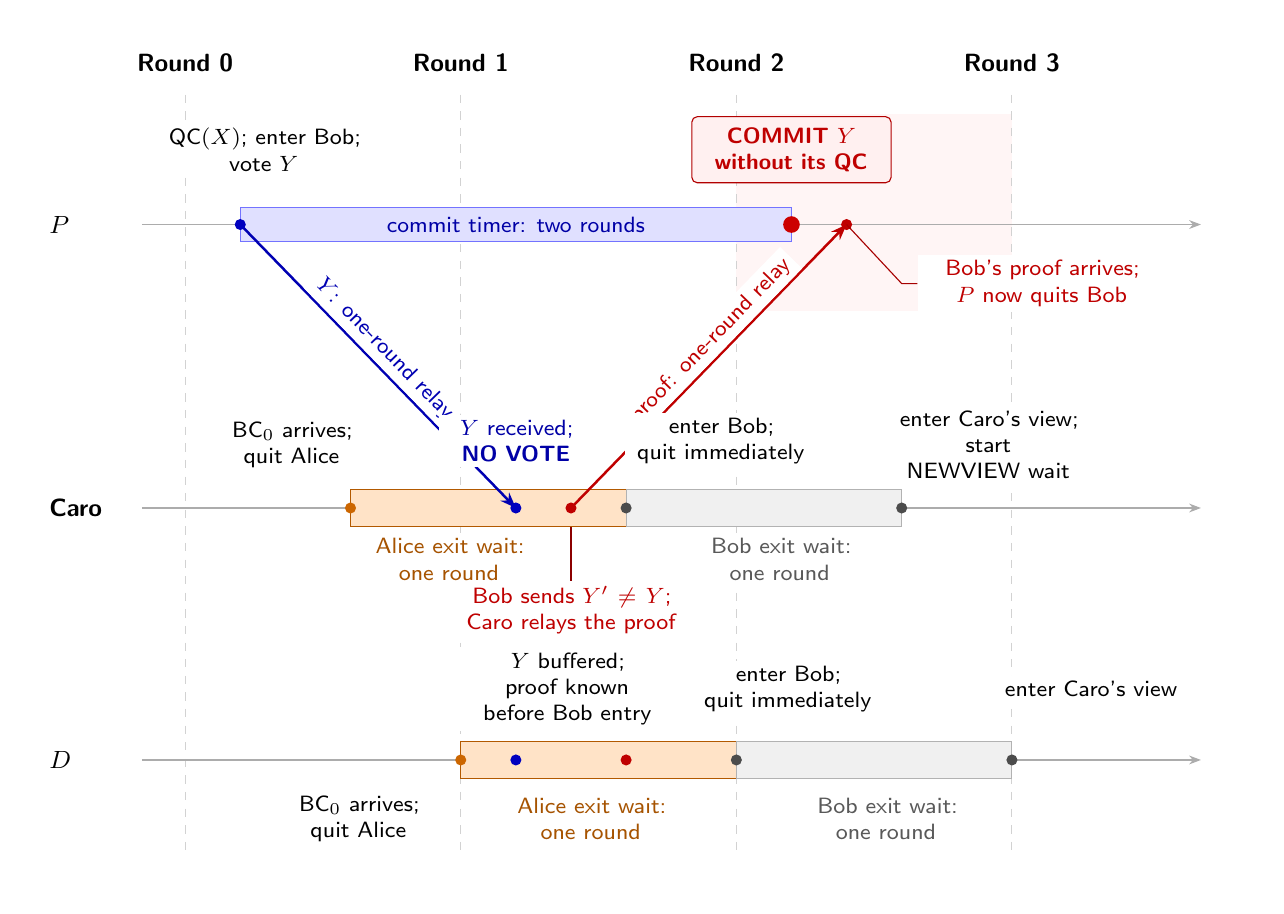
\begin{tikzpicture}[x=1cm,y=-1cm,font=\sffamily\footnotesize,
  msg/.style={-{Stealth[length=2mm]},line width=.9pt},
  note/.style={align=center,fill=white,inner sep=2pt},
  attackdot/.style={circle,inner sep=0pt,minimum size=4pt},
  labelbox/.style={note,rounded corners=2pt,draw,inner sep=4pt}]
\path[use as bounding box] (-.1,-.1) rectangle (15.5,10.8);
% Round boundaries and replica lifelines.
\fill[red!4] (8.9,1.0) rectangle (12.4,3.5);
\foreach \x/\r in {1.9/0,5.4/1,8.9/2,12.4/3}{
  \draw[gray!35,dashed] (\x,.75) -- (\x,10.4);
  \node[font=\sffamily\bfseries\small] at (\x,.35) {Round \r};
}
\foreach \y/\who in {2.4/{$P$},6.0/{Caro},9.2/{$D$}}{
  \node[anchor=west,font=\sffamily\bfseries\small] at (.05,\y) {\who};
  \draw[-{Stealth[length=1.5mm]},gray!65] (1.35,\y) -- (14.8,\y);
}
% Timers and exit waits.  Equal widths denote equal durations.
\filldraw[fill=blue!12,draw=blue!55] (2.6,2.18) rectangle (9.6,2.62);
\node[text=blue!65!black] at (6.1,2.4) {commit timer: two rounds};
\filldraw[fill=orange!22,draw=orange!70!black] (4.0,5.76) rectangle (7.5,6.24);
\filldraw[fill=gray!12,draw=gray!60] (7.5,5.76) rectangle (11.0,6.24);
\filldraw[fill=orange!22,draw=orange!70!black] (5.4,8.96) rectangle (8.9,9.44);
\filldraw[fill=gray!12,draw=gray!60] (8.9,8.96) rectangle (12.4,9.44);
% Selected messages: each diagonal below spans exactly one round.
\draw[msg,blue!70!black] (2.6,2.4) --
  node[note,sloped,above,pos=.48,text=blue!70!black] {$Y$: one-round relay}
  (6.1,6.0);
\draw[msg,red!75!black] (6.8,6.0) --
  node[note,sloped,above,pos=.55,text=red!75!black] {proof: one-round relay}
  (10.3,2.4);
% P: the wrong commit strictly precedes receipt of Bob's proof.
\node[attackdot,fill=blue!75!black] at (2.6,2.4) {};
\node[note,text width=2.65cm] at (2.9,1.45)
  {$\QC(X)$; enter Bob;\\vote $Y$};
\node[attackdot,fill=red!80!black,minimum size=6pt] at (9.6,2.4) {};
\node[labelbox,draw=red!70!black,fill=red!6,text=red!75!black,
  text width=2.25cm,font=\sffamily\bfseries\footnotesize] at (9.6,1.45)
  {COMMIT $Y$\\without its QC};
\node[attackdot,fill=red!75!black] at (10.3,2.4) {};
\draw[red!65!black] (10.3,2.4) -- (11.0,3.15) -- (11.2,3.15);
\node[note,anchor=west,text width=3.0cm,text=red!75!black] at (11.2,3.15)
  {Bob's proof arrives;\\$P$ now quits Bob};
% Caro: receives Y before it is allowed to vote; sees proof before entry.
\node[attackdot,fill=orange!80!black] at (4.0,6.0) {};
\node[note,text width=2.15cm] at (3.25,5.2) {$\BC_0$ arrives;\\quit Alice};
\node[attackdot,fill=blue!75!black] at (6.1,6.0) {};
\node[note,text width=1.8cm,text=blue!65!black] at (6.1,5.15)
  {$Y$ received;\\\textbf{NO VOTE}};
\node[note,text width=2.55cm,text=orange!65!black] at (5.25,6.65)
  {Alice exit wait: one round};
\node[attackdot,fill=red!75!black] at (6.8,6.0) {};
\draw[red!55!black] (6.8,6.24) -- (6.8,7.0);
\node[note,text width=3.0cm,text=red!75!black] at (6.8,7.3)
  {Bob sends $Y'\ne Y$;\\Caro relays the proof};
\node[attackdot,fill=black!70] at (7.5,6.0) {};
\node[note,text width=2.3cm] at (8.7,5.15)
  {enter Bob;\\quit immediately};
\node[note,text width=2.6cm,text=black!65] at (9.45,6.65)
  {Bob exit wait: one round};
\node[attackdot,fill=black!70] at (11.0,6.0) {};
\node[note,text width=2.65cm] at (12.1,5.2)
  {enter Caro's view;\\start NEWVIEW wait};
% D: its Alice wait starts one round later than Round 0's boundary.
\node[attackdot,fill=orange!80!black] at (5.4,9.2) {};
\node[note,text width=2.1cm] at (4.1,9.95) {$\BC_0$ arrives;\\quit Alice};
\node[attackdot,fill=blue!75!black] at (6.1,9.2) {};
\node[attackdot,fill=red!75!black] at (7.5,9.2) {};
\node[note,text width=2.8cm] at (6.75,8.3)
  {$Y$ buffered; proof known\\before Bob entry};
\node[note,text width=3.0cm,text=orange!65!black] at (7.05,9.95)
  {Alice exit wait: one round};
\node[attackdot,fill=black!70] at (8.9,9.2) {};
\node[note,text width=2.25cm] at (9.55,8.3)
  {enter Bob;\\quit immediately};
\node[note,text width=2.7cm,text=black!65] at (10.8,9.95)
  {Bob exit wait: one round};
\node[attackdot,fill=black!70] at (12.4,9.2) {};
\node[note,text width=2.4cm] at (13.4,8.3) {enter Caro's view};
\end{tikzpicture}
\end{center}
\vspace{-5pt}
\textit{Selected messages are drawn. $P$ also relays $Y$ to $D$ early in
Round~1; Caro's proof reaches $D$ later in that round. Alice's late quit
proof cancels only $P$'s Alice-view timer.}

\medskip
\textbf{B. Highest-QC recovery preserves $X$, but cannot protect uncertified $Y$.}
\begin{center}
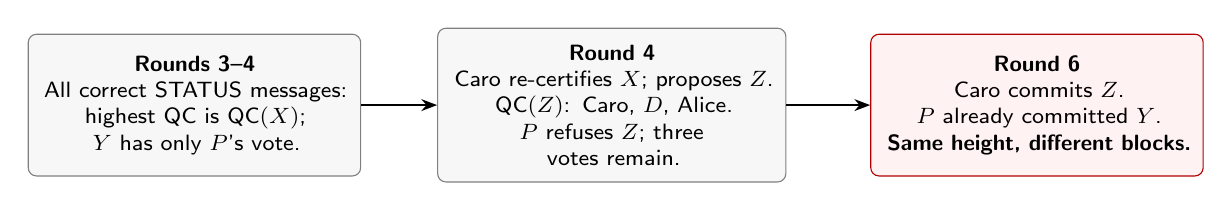
\begin{tikzpicture}[x=1cm,y=1cm,font=\sffamily\footnotesize,
  attackstage/.style={draw=black!50,rounded corners=3pt,fill=black!3,
    align=center,inner sep=6pt,minimum height=1.8cm},
  flow/.style={-{Stealth[length=2mm]},line width=.8pt}]
\node[attackstage,text width=3.8cm] (status) at (2.1,0)
  {\textbf{Rounds 3--4}\\All correct STATUS messages:\\highest QC is $\QC(X)$;\\$Y$ has only $P$'s vote.};
\node[attackstage,text width=4.0cm] (recover) at (7.4,0)
  {\textbf{Round 4}\\Caro re-certifies $X$; proposes $Z$.\\$\QC(Z)$: Caro, $D$, Alice.\\$P$ refuses $Z$; three votes remain.};
\node[attackstage,draw=red!70!black,fill=red!5,text width=3.8cm] (conflict) at (12.8,0)
  {\textbf{Round 6}\\Caro commits $Z$.\\$P$ already committed $Y$.\\\textbf{Same height, different blocks.}};
\draw[flow] (status) -- (recover);
\draw[flow] (recover) -- (conflict);
\end{tikzpicture}
\end{center}

\textbf{Failure point:} $Y$ has no QC when $P$'s timer expires.
This plot concerns the previous per-view-cancellation candidate. The new
global-abort rule cancels this timer before expiry; requiring $\QC(Y)$ at
commit is a separate way to block the same historical trace.

\begin{thebibliography}{1}\small
\bibitem{sync}
I. Abraham, D. Malkhi, K. Nayak, L. Ren, and M. Yin.
\emph{Sync HotStuff: Simple and Practical Synchronous State Machine Replication}.
IEEE Symposium on Security and Privacy, 2020, Section II, Figures 1--2.
\href{https://conferences.computer.org/sp/pdfs/sp/2020/349700a106.pdf}{Published paper}.
\end{thebibliography}
\end{document}
